\section{Implementation}
\label{sec:implementation}
We briefly describe here the implementation of P2Pedia. It is important to note that as P2Pedia is conceptually defined with respect to an abstract model of file-sharing, its functionality could be implemented over other P2P architectures as well.

\subsection{U-P2P}

P2Pedia is implemented using the Universal Peer-to-Peer (U-P2P) framework \cite{UP2P2002, UP2PSemelsJournal2009, UP2P:201101TechReport}. 

The architecture of U-P2P is illustrated in Figure \ref{fig:TSarchitecture}.
\begin{figure}[htb]
	\centering
		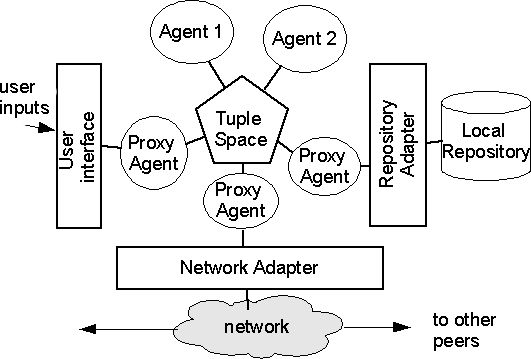
\includegraphics[scale=0.5]{U-P2Parchitecture.png}
	\caption{Architecture of U-P2P}
	\label{fig:TSarchitecture}
\end{figure}

The user interface of U-P2P is implemented with Java ServerPages and Servlets, and uses the Apache Tomcat Servlet Engine. Apache Xindice is used as the local XML database, and the Network Adapter uses a Java implementation of the Gnutella protocol. These three components are coordinated using a tuple space, which allows for asynchronous ad-hoc coordination, and seamless extension of the system functionality: additional components can be simply plugged into the tuple-space and make use of the file-sharing ``primitives" implemented by the main components. Graph query processing is implemented in this way, as described in the next section.

The Wiki functionality is implemented in Javascript using the JSCreole parser\footnote{http://jscreole.sf.net}.

\subsection{Implementation of Graph Queries}

As we have described in Section \ref{sec:ancestry}, U-P2P supports simple path queries over the graph of documents, and path queries using the transitive closure of an edge label.

We briefly describe here the implementation of path query answering in U-P2P. Our approach relies on multiple ``agents" generated on the fly from the query definition, and coordinated through the tuple space. For a path query defined by the path $\pi = l_1,l_2 \dots, l_k$ and the input document $D$, one agent is generated to process the sub-queries associated with each of the edge labels $l_i$. 

Starting from the input document $D$, the first ``agent"  must find all documents related to $D$ by an edge labelled $l_1$. Due to the asynchronicity of the P2P search protocol, the answers returned for this subquery arrive asynchronously in the tuple-space, and it is not known when the last answer has arrived (i.e. the termination can not be detected with certainty). The agent associated with $l_2$ asynchronously collects the answers from the previous subquery, and for each answer $d_{i}$ outputs a subquery to find documents related to $d_{i}$ by an edge labelled $l_2$. The answers to all of these subqueries are in turn collected by the next agent down the line, and in this way the different matching paths are explored in parallel to provide the answers to the overall path query.

The same processing can be slightly modified to answer a transitive closure query: a single agent is used, which recursively reuses the answers to its own subqueries. For a query to find the ancestors of some document $D_0$, i.e. documents related to $D_0$ by paths matching the transitive closure of the label ``parent", a single agent queries for the ``parent" documents of $D_0$, then for the parents of the answer documents, and this way recursively, until there are no more answers. Again, termination cannot be detected due to the asynchronicity of the search, so the searching agent remains active until the user runs a new query or closes the query answer page.

\subsection{Implementation of Trust Indicators}

The trust indicators in P2Pedia are either implemented by attaching additional meta-data to search response messages, or by extracting information included in the standard Gnutella protocol messages.
\paragraph*{Jaccard Index} When responding to a query the responding node includes a list of the documents it stores (only their identifiers), which the querying node can then use to calculate the Jaccard Index of the two sets. This increases the size of the messages and therefore constitutes a slight overhead.
\paragraph*{Network Distance} This value is determined by the querying node when receiving a search response by checking the Gnutella protocol ``hops" value on the incoming response. 
\paragraph*{Peer Popularity} The number of incoming connections to a node is included as meta-data in search responses. Note that this could be falsified by the node. Methods to infer the network topology by analyzing message hops should be explored to address this issue.
\paragraph*{Document Popularity} No additional meta-data is required for this indicator, as a querying node simply tracks the number of query hits it receives for a specific document. 

\subsection{On the Possibility of Deploying this System over a DHT}
As we have noted, this design could work on different insfrastructures. Most existing distributed wikis use DHTs to optimize the storage and access time of the documents. However, in our particular approach, the benefits of DHT would be much less important.
First, the principle of the system is that users freely maintain any version they like. Therefore storing all the versions according to a DHT protocol goes against this principle.

Secondly, we could consider using a DHT to optimize queries, following the idea of Emule, which uses the Kad DHT to support its query index. The problem here would be that the index would be huge, since the system is focused on text. The Emule approach is to index file names : for each work in a file name, place an index entry to the file in the appropriate DHT node. This implies that there exist perhaps at most 5 or 6 pointers for each file. In our case, as we support full-text search, we would need to index each word appearing in the document, and we would therefore need potentially hundreds of pointers to each file, which implies a very large index structure, that would imply major processing overhead.
